\documentclass{report}

\input{preamble}
\input{macros}
\input{letterfonts}

\title{\Huge{Math 244}}
\author{\huge{PSET 2}}
\date{Feb 3 2025}

\begin{document}

\maketitle
\newpage% or \cleardoublepage
% \pdfbookmark[<level>]{<title>}{<dest>}
\pdfbookmark[section]{\contentsname}{toc}
\tableofcontents
\pagebreak

\section*{Section 1.5 Problem 5}
\addcontentsline{toc}{section}{Problem 1}

\qs{}{
  Prove the associativity of composing relations: If $R$, $S$, and $T$ are relations such that 
  $( R \circ S) \circ T$ is well defined, then $R \circ (S \circ T)$ is well defined and equal to $( R \circ S) \circ T$.
}


\begin{proofWithHibiscus}
  Suppose $(w,z)$ lies in $(R \circ S) \circ T$ 

  If $(w, y) \in R \circ S$, there is some $x$ such that 

  \[ (w,x) \in R \quad \text{and} \quad (x,y) \in S. \]

  Since we also have $(y,z) \in T$, so $(x, z) \in S \circ T$. 

  We now have $(w,x) \in R$ and $(x,z) \in S \circ T$, which means that $(w,z) \in R \circ (S \circ T)$. 

  This means  
  \[ (R \circ S) \circ T \subseteq R \circ (S \circ T). \]

  Now, for the reverse inclusion, suppose $(w,z) \in R \circ (S \circ T)$. Then there exists some $x$ such that 
  \begin{itemize}
    \item [1] $(w,x) \in R$, and 
    \item [2] $(x,z) \in S \circ T$. 
  \end{itemize}

  Since $(x, z) \in S \circ T$, there is some $y$ such that 

  \[ (x,y) \in S \quad \text{and} \quad (y,z) \in T. \]

  Since $(w,x) \in R$ and $(x,y) \in S$, we conclude that $(w,y) \in R \circ S$. 

  Since we also have $(y,z) \in T$, that means $(w,z) \in (R \circ S) \circ T$. \\ 
   
  So 
  \[ R \circ (S \circ T) \subseteq (R \circ S) \circ T. \]

  So  
  \[ (R \circ S) \circ T = R \circ (S \circ T). \]

\end{proofWithHibiscus}

\section*{Section 1.6 Problem 3}
\addcontentsline{toc}{section}{Problem 2}

\qs{}{
  Prove that a relation $R$ is transitive if and only if $R \circ R \subseteq R$.
}

\begin{keyideaWithLotus}
  We need to show 
  \begin{itemize}
    \item [$\Rightarrow$] If $R$ is transitive, then, $R \circ R \subseteq R$
    \item [$\Leftarrow$] If $R \circ R \subseteq R$, then $R$ is transitive.   
  \end{itemize}

\end{keyideaWithLotus}

\begin{RemarkWithLily}{$\Rightarrow$}
  WWe assume that $R$ is transitive. \\
  By def or relational composition we know that for a pair $(a,c) \in R \circ R$ there exists some $b$ $s.t.$ 

  \[ (a,b) \in R \quad \text{and} \quad (b,c) \in R \]

  Since $(a,b) \in R$ and $(b,c) \in R$, and $R$ is transitive
  \[ (a,c) \in R \]
  
  So every pair in $R \circ R \subseteq R$   
\end{RemarkWithLily}

\begin{RemarkWithLily}{$\Leftarrow$}
  WWe asume $R \circ R \subseteq R$ \\
  $R$ is transitive \textit{iff} for all $a,b,c$ 
  \[ (a,b) \in R \quad \text{and} \quad (b,c) \in R \]
  so, 
  \[ (a,c) \in R \]
  Now we suppose $(a,b) \in R $ and $(b,c)$ in R which would make $b$ the intermediate element so 
  \[ (a,c) \in R \circ R \]
  from our assumption any pair in $R \circ R$ has to be in $R$
  \[ (a,c) \in R \]     
\end{RemarkWithLily}

\section*{Section 1.6 Problem 6}
\addcontentsline{toc}{section}{Problem 3}

\qs{}{
  Describe all relations on a set $X$ that are equivalences and orderings at the same time. 
}


\begin{RemarkWithLily}{For Prob 3}
  FFor this to be the case reflexivity and transitivity are required but for equivalence symmetry is required while for 
  ordering antisymmetry is required.    
  \bigskip 
  IF $R$ is symmetric and antisymmetric, for any $x,y \in X$
  \begin{itemize}
    \item [1] $xRy$ and $yRx$ for symmetry 
    \item [2] $x=y$ for antisymmetry
  \end{itemize}                    
  Meaning that if $xRy$ holds than $x$ and $y$ have to be the same element. So really the relation is relating an element 
  to itself 
  
  \bigskip 
  \[ R = \{ (x,x) : x \in X \}\] 
\end{RemarkWithLily}

\newpage 

\section*{Section 2.1 Problem 4}
\addcontentsline{toc}{section}{Problem 4}


\qs{}{
  Let $(X, \preceq)$, $(Y, \preceq)$ be ordered sets. We say that they are \textit{isomorphic} if there exists a bijection $f: X \to Y$ such that for every $x, y \in X$, we have 
  $x \leq y$ if and only if $f(x) \preceq f(y)$. 

  \begin{itemize}
    \item [a)] Draw Hasse diagrams for all non-isomorphic ordered sets with 3 elements posets.
    \item [b)] Prove that any two $n$-elements linearly ordered sets are isomorphic.
  \end{itemize}
}

\subsection*{Prob 4.a}
\addcontentsline{toc}{subsection}{Prob 4.a}


\begin{center}
  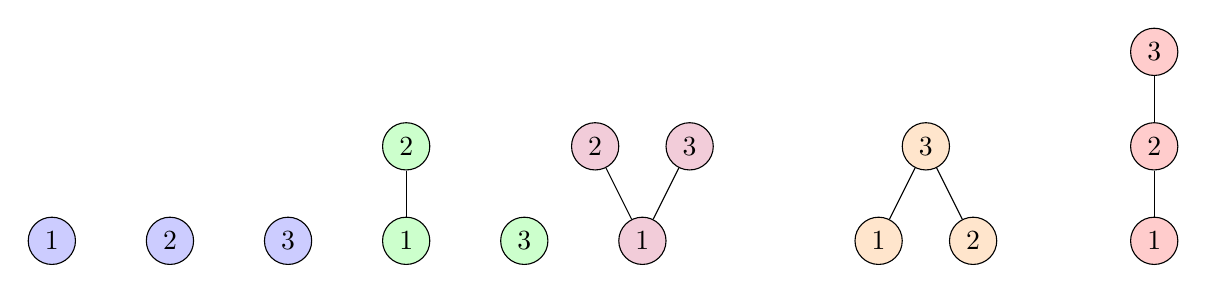
\begin{tikzpicture}[scale=1, every node/.style={circle, draw, minimum size=6mm, inner sep=2pt}]
    % --- Diagram 1: Antichain ---
    \node[fill=blue!20] (A1) at (0,0) {1};
    \node[fill=blue!20] (B1) at (1.5,0) {2};
    \node[fill=blue!20] (C1) at (3,0) {3};
    
    % --- Diagram 2: 2+1 (a 2–chain with an isolated point) ---
    \node[fill=green!20] (A2) at (4.5,0) {1};
    \node[fill=green!20] (B2) at (4.5,1.2) {2};
    \node[fill=green!20] (C2) at (6,0) {3};
    \draw (A2) -- (B2);
    
    % --- Diagram 3: V–poset (one minimal element below two incomparable elements) ---
    \node[fill=purple!20] (A3) at (7.5,0) {1};
    \node[fill=purple!20] (B3) at (6.9,1.2) {2};
    \node[fill=purple!20] (C3) at (8.1,1.2) {3};
    \draw (A3) -- (B3);
    \draw (A3) -- (C3);
    
    % --- Diagram 4: Λ–poset (dual of the V–poset) ---
    \node[fill=orange!20] (A4) at (10.5,0) {1};
    \node[fill=orange!20] (B4) at (11.7,0) {2};
    \node[fill=orange!20] (C4) at (11.1,1.2) {3};
    \draw (A4) -- (C4);
    \draw (B4) -- (C4);
    
    % --- Diagram 5: Chain (totally ordered 3–chain) ---
    \node[fill=red!20] (A5) at (14,0) {1};
    \node[fill=red!20] (B5) at (14,1.2) {2};
    \node[fill=red!20] (C5) at (14,2.4) {3};
    \draw (A5) -- (B5);
    \draw (B5) -- (C5);
    
  \end{tikzpicture}
\end{center}

\subsection*{Prob 4.b}
\addcontentsline{toc}{subsection}{Prob 4.b}

\begin{keyideaWithLotus}
  We want to show that if $(X, \leq)$ and $(Y, \preceq)$ are two linearly ordered sets with $n$ elements, then they must be isomorphic.
\end{keyideaWithLotus}

\begin{basecaseWithPoppy}
  $n = 1$

  If $X$ and $Y$ both have exactly one element, say $X = \{x\}$ and $Y = \{y\}$, we can define the function 
  \[
  h(x) = y.
  \]
  This is clearly a bijection since both sets have only one element, and there is no ordering to worry about. Since order is trivially preserved, $X$ and $Y$ are isomorphic.
\end{basecaseWithPoppy}

\begin{inducthypWithRose}
  Assume that for any two linearly ordered sets with $n-1$ elements, there exists an order-preserving bijection (an isomorphism) between them.
\end{inducthypWithRose}

\begin{inductstepWithTulip}

  Suppose $X$ and $Y$ are two linearly ordered sets with $n$ elements. Since the order is total, each set has a unique largest element. Let
  \[ x_{\text{max}} = \text{largest element of } X, \quad y_{\text{max}} = \text{largest element of } Y. \]
  
  Now, consider the subsets
  \[ X' = X \setminus \{x_{\text{max}}\}, \quad Y' = Y \setminus \{y_{\text{max}}\}. \]
  These are both linearly ordered sets with $n-1$ elements. By the inductive hypothesis, there exists an isomorphism 
  \[ g: X' \to Y'. \]

  Let $f: X \to Y$ be 
  \[
  f(x)=
  \begin{cases}
  g(x) & \text{if } x \in X',\\[1mm]
  y_{\text{max}} & \text{if } x = x_{\text{max}}.
  \end{cases}
  \]

  Since $g$ is a bijection from $X'$ to $Y'$ and $y_{\text{max}}$ is not in the image of $g$, the function $f$ is one-to-one and onto.

  \bigskip

  If both $x_1$ and $x_2$ are in $X'$, then $f(x_1)=g(x_1)$ and $f(x_2)=g(x_2)$, and since $g$ is order preserving, the order is maintained. \\ 
  If $x_1 \in X'$ and $x_2 = x_{\text{max}}$, then in $X$ we have $x_1 \leq x_{\text{max}}$. In $Y$, since $y_{\text{max}}$ is the largest, $g(x_1) \preceq y_{\text{max}}$, so the order is preserved. \\
  Finally, if both $x_1 = x_{\text{max}}$ and $x_2 = x_{\text{max}}$, the order obviously holds.

  \medskip

  Since $f$ is a bijection and it preserves the order, it is an isomorphism. 

  \medskip

  By the principle of induction, the claim holds for all $n$.

\end{inductstepWithTulip}


\section*{Section 2.2 Problem 3}
\addcontentsline{toc}{section}{Problem 5}

\qs{}{
  \begin{itemize}
    \item [a)] Consider the set $\{ 1, 2, \ldots n \}$ ordered by the divisibility relation $|$. What is the maximum possible number of elements of a set $X \subseteq \{1, 2, \ldots n \}$ that is ordered linearly by the relation $|$ 
    \item [b)] Solve the same question for the set $2^{\{1, 2, \ldots n\}}$ ordered by the inclusion relation $\subseteq$.
  \end{itemize}
}

\subsection*{Prob 5.a}
\addcontentsline{toc}{subsection}{Prob 5.a}

\begin{RemarkWithLily}{Prob 5.a }
  IIt is 1 + the longest branch of the prime facorization of n . 
\end{RemarkWithLily}

\subsection*{Prob 5.b}
\addcontentsline{toc}{subsection}{Prob 5.b}

\begin{RemarkWithLily}{Prob 5.b}
  AA chain in $2^{\{1, 2, \ldots n\}}$ would be a collection of subsets $S_{1} \subset S_{2} \subset \ldots \subset  S_{k}$
  If two distinct subsets have the same number of elements, then none could be a proper subset of the other. So the sizes of subsequent subsets must be strictly increasing.  

  \bigskip 
  Since any subset of $\{1,2,\dots,n\}$ has a cardinality between $0$ and $n$, there can be at most $n+1$ different cardinalities. 
  
\end{RemarkWithLily}

\newpage 

\section*{Optionl Bonus Problem}
\addcontentsline{toc}{section}{Bonus Problem}

\qs{}{
  Let le$(X,  \preceq )$ denote teh number of linear extensions of a partially ordered set $(X , \preceq)$. Prove: 
  \begin{itemize}
    \item [a)] le$(X, \preceq) = 1$ if and only if $(X, \preceq)$ is a linear ordering.
    \item [b)] le$(X, \preceq) \leq n!$, where $n = |X|$    
  \end{itemize}
}

\subsection*{Bonus Prob Part a}
\addcontentsline{toc}{subsection}{Bonus Prob A}

\begin{proofWithHibiscus}
  (\(\Rightarrow\)) Suppose that $\operatorname{le}(X, \preceq) = 1$. 

  \bigskip
  
  Assume, for contradiction, that $(X, \preceq)$ is not a linear order. Then there exist two distinct elements 
  $a, b \in X$ such that neither $a \preceq b$ nor $b \preceq a$ holds. But in linear extensions every pair of elements must be comparable. So two cases 
  \begin{enumerate}
    \item One linear extension where $a$ comes before $b$ 
    \item or one where $b$ comes before $a$ .
  \end{enumerate}
  This would make two distinct linear extensions, contradicting the assumption. $\preceq$ must be a total order.

  \bigskip
  
  (\(\Leftarrow\)) Suppose that $(X, \preceq)$ is a linear total order. We need to show that $\operatorname{le}(X, \preceq) = 1$.

  \bigskip
  
  Since $\preceq$ is already a total order, it already orders every pair of elements in $X$. The only possible linear extension is the order $\preceq$ itself. So, there is exactly one linear extension. $\operatorname{le}(X, \preceq) = 1$.
\end{proofWithHibiscus}

\subsection*{Bonus Prob Part B}
\addcontentsline{toc}{subsection}{Bonus Prob B}


\begin{proofWithHibiscus}
  A linear extension of $(X, \preceq)$ is  a total order on $X$ that respects the partial order. A total order on a finite set $X$ with $n$ elements would be a permutation of $X$ and there are $n!$ permutations of a set with $n$ elements. 

  But not every permutation of $X$ will be a linear extension of $(X, \preceq)$ because the permutation must respect the partial order $\preceq$. So, the set of linear extensions is a subset of the set of all permutations of $X$.

  \[ \operatorname{le}(X, \preceq) \leq n! \]

\end{proofWithHibiscus}



\end{document}